The \textbf{V}enios\textbf{E}nergy\textbf{P}latform is a cloud application
developed and hosted by Venios. The customers are grid operators who can use
it to visualize the grid, track real time data, have it predict 
operational parameters such as prosumer loads and control the grid.
The long term aim of this project is to develop an algorithm that takes in
congested grid areas as its input and advises VEP on possible improved
switch states and their effects. This dissertation aims to implement the first step of this
process by taking in grid data from VEP and analysing it, trying to figure out
improved grid configurations. Data obtained for this project from VEP can broadly
be categorized
into topological and load profiles. Whilst the former is anything having to do with
the grid structure, its geographical location and its operating parameters the later
are production or consumption values over time for each of the prosumers.\\
All data is obtained over Venios' API, in json format. This means any
grid area of any VEP customer can be used for this analysis just by changing out
the request parameters and use of the relevant authorization tokens for that customer.
No code changes are required. This approach has the added advantage that any customer grid
data is only stored in memory and only temporarily on the machine running the analysis. This
has data privacy advantages.

\subsection{Data exchanged}

Data elements in VEP are identified by their \texttt{ForeignKey} (abbrv. to \texttt{FK}). This is a unique key which
uniquely identifies the element and is sufficient to retrieve it. Data retrieved from the API might
be a combination of many data elements and might therefore not have a single \texttt{ForeignKey}, however
it might mention other elements by their \texttt{ForeignKey} so that they can be retrieved.

\subsubsection{API methods}

\begin{tabular}{ l  p{12cm}} 
    \hline
    \multicolumn{2}{c}{\textbf{Voltage Groups}}\\
    \hline
    Method Name     & \texttt{GetAllVoltageGroups} \\
    Input           & -\\
    Output          & \texttt{list of VoltageLevel} \\
    Description     & Returns all voltage levels available in the current VEP instance. A voltage level is a level within the grid, normal households are usually connected to the LV (low voltage) voltage level at 400V\\
\end{tabular}

\vspace{.5cm}

\begin{tabular}{ l  p{12cm}} 
    \hline
    \multicolumn{2}{c}{\textbf{Grids in Geographical Boundary}}\\
    \hline
    Method Name     & \texttt{LoadGridsInGeoBounds} \\
    Input           & \texttt{VoltageLevel, GeoBounds}\\
    Output          & \texttt{list of GridFK}\\
    Description     & Returns foreign keys to grids within a geographical boundary and voltage level. A "grid" in vep is an administrative set of grid components usually connected to one transformer\\
\end{tabular}

\vspace{.5cm}

\begin{tabular}{ l  p{12cm}} 
    \hline
    \multicolumn{2}{c}{\textbf{Conducting Topology}}\\
    \hline
    Method Name     & \texttt{LoadManyConductingTopologies} \\
    Input           & \texttt{list of GridFK}\\
    Output          & \texttt{GridTopology} \\
    Description     & Returns the conducting topology of a grid, these are its cables, nodes and transformers\\
\end{tabular}

\vspace{.5cm}

\begin{tabular}{ l  p{12cm}} 
    \hline
    \multicolumn{2}{c}{\textbf{Get Many}}\\
    \hline
    Method Name     & \texttt{GetMany} \\
    Input           & \texttt{list of FK}\\
    Output          & Raw VEP data element \\
    Description     & Used to retrieve a list of VEP data elements of any data type. Used here to retrieve transformer and cable specifications\\
\end{tabular}

\vspace{.5cm}

\begin{tabular}{ l  p{12cm}} 
    \hline
    \multicolumn{2}{c}{\textbf{Load Profiles}}\\
    \hline
    Method Name     & \texttt{GetLoadProfiles} \\
    Input           & \texttt{list of ProsumerFK, start datetime, end datetime, resolution, model prefrences}\\
    Output          & list of complex Power values \\
    Description     & Returns a load values over time from a start datetime to an end datetime with the resolution specified. If multiple models to generate load profiles are available a preferred model can be specified \\
\end{tabular}

\subsubsection{Complex data types}

Below is a description of the relevant complex data types retrieved from VEP. This is an incomplete
description only showing relevant data fields.

\vspace{.5cm}

\begin{tabular}{ l p{3cm} l p{8cm}} 
    \hline
    \multicolumn{4}{c}{\texttt{VoltageLevel}}\\
    \hline
    \textbf{Field Name} & \textbf{Data Type}       & \textbf{Unit} & \textbf{Description} \\
    \hline
    LowerLimit          & \texttt{double}          & $V$           & Lower voltage limit of this voltage level\\
    UpperLimit          & \texttt{double}          & $V$           & Upper voltage limit of this voltage level\\
    ForeignKey          & \texttt{ForeignKey}      &               & \texttt{ForeignKey} of this voltage level
\end{tabular}

\vspace{.5cm}

\begin{tabular}{ l p{3cm} l p{8cm}} 
    \hline
    \multicolumn{4}{c}{\texttt{GridTopology}}\\
    \hline
    \textbf{Field Name} & \textbf{Data Type}              & \textbf{Unit} & \textbf{Description} \\
    \hline
    GridFK              & \texttt{ForeignKey}                       &               & \texttt{ForeignKey} of the grid\\
    Transformer         & \texttt{list of GridElement}    &         & All transformers of the grid\\
    Edges               & \texttt{list of GridElement}    &         & All edges of the grid (without transformers which are also an edge in VEP)\\
    Nodes               & \texttt{list of GridElement}    &         & All nodes of the grid \\
\end{tabular}

\vspace{.5cm}

\begin{tabular}{ l p{3cm} l p{8cm}} 
    \hline
    \multicolumn{4}{c}{\texttt{GridElement}}\\
    \hline
    \textbf{Field Name} & \textbf{Data Type}            & \textbf{Unit} & \textbf{Description} \\
    \hline
    PrimaryKey          & \texttt{ForeignKey}           &               & The primary key of the corresponding VEP data element\\
    Name                & \texttt{string}               &               & Name of the element given by the grid operator\\
    \hline
    \multicolumn{4}{c}{\textbf{if edge}}\\
    \hline
    NodeA               & \texttt{ForeignKey}           &               & Node connected on side A\\
    NodeB               & \texttt{ForeignKey}           &               & Node connected on side B\\
    \hline
    \multicolumn{4}{c}{\textbf{if Cable or Transformer}}\\
    \hline
    Specs               & \texttt{list of SpecificationFK}             &               & \texttt{ForeignKey} to the specification specifying physical parameters of the transformer or cable\\
    \hline
    \multicolumn{4}{c}{\textbf{if Cable}}\\
    \hline
    Length              & \texttt{double}              &  $m$          & Length of the cable\\
    \hline
    \multicolumn{4}{c}{\textbf{if Switch}}\\
    \hline
    DefaultSwitchState  & \texttt{boolean}             &               & True if the switch is closed in the default configuration\\
    CurrentSwitchState  & \texttt{boolean}             &               & True if the switch is currently closed\\
\end{tabular}

\vspace{.5cm}

\begin{tabular}{ l p{3cm} l p{8cm}} 
    \hline
    \multicolumn{4}{c}{\texttt{Cable Specification}}\\
    \hline
    \textbf{Field Name} & \textbf{Data Type}        & \textbf{Unit} & \textbf{Description} \\
    \hline
    NominalCurrent      & \texttt{double}           & $A$           & Max. operating current in amps\\              
    Resistance20        & \texttt{double}           & $\Omega/m$    & Resistance at $20C^\circ$\\  
    Reactance           & \texttt{double}           & $\Omega/m$    & Reactance\\              
\end{tabular}

\begin{tabular}{ l p{3cm} l p{8cm}} 
    \hline
    \multicolumn{4}{c}{\texttt{Transformer Specification}}\\
    \hline
    \textbf{Field Name} & \textbf{Data Type}        & \textbf{Unit} & \textbf{Description} \\
    \hline
    RatedPower          & \texttt{double}           & $VA$          & Max. operating power\\              
   \end{tabular}

\vspace{1cm}

\subsection{Topological grid data}

The grid data coming from VEP contains edges and nodes. For each there are various subtypes, with some relevance
to this work.\\
\\
The following node types are relevant:
\begin{itemize}
    \item \textbf{Domestic Prosumer} household, usually consumes power
    \item \textbf{Industry Prosumer} stores, factories, etc.
    \item \textbf{Solar Panel}, injecting power into the grid
    \item \textbf{Battery Storage}, temporarily stores power and later injects it
    \item \textbf{Electric car chargers}
    \item \textbf{Other Prosumer} other types of prosumers like, wind turbines, electric heaters, heat pumps etc. 
    \item \textbf{Any other node} does not inject or consume power, and thus only modelled as a junction between edges
\end{itemize}

Then there are the following edge types:

\begin{itemize}
    \item \textbf{Cable} A cable with actual length, resistance and reactance
    \item \textbf{Transformer} Connects different voltage levels, here not modelled, instead the node its connected to, becomes the slack node
    \item \textbf{Switch} Connects two nodes and can be interrupted. Modelled with zero resistance and reactance
    \item \textbf{Any other edge} other short miscellaneous edges connecting nodes within substations or electrical cabinets. Modelled as zero resistance and reactance
\end{itemize}

A good dataset for validation and comparison is the SimBench data set. It is a set of
gird data provided by the University Kassel. The dataset aims to model typical German
grids in rural and urban environments. It was specifically designed to include a higher
number of renewables in the low voltage level, like solar panels\autocite{simbench}. These
simbench grids can be also imported in VEP and where thus used as the initial validation case
for this work.\\

Figure \ref{fig:vep:simbench_node_types} shows one of these Simbench grids ("1-LV-rural1"). 
Within VEP this grid is modelled with 553 edges and 553 nodes. A lot of these nodes are there to model
internals like bus bars or protective switch setups. For powerflow and for analysing
switch states these nodes can be merged down to 96 with 95 edges running between them. 
The exact method to do so will be explained in the data preparation section. These numbers of nodes
are typical for German grids\autocite{venios}.

\begin{figure}[H]
    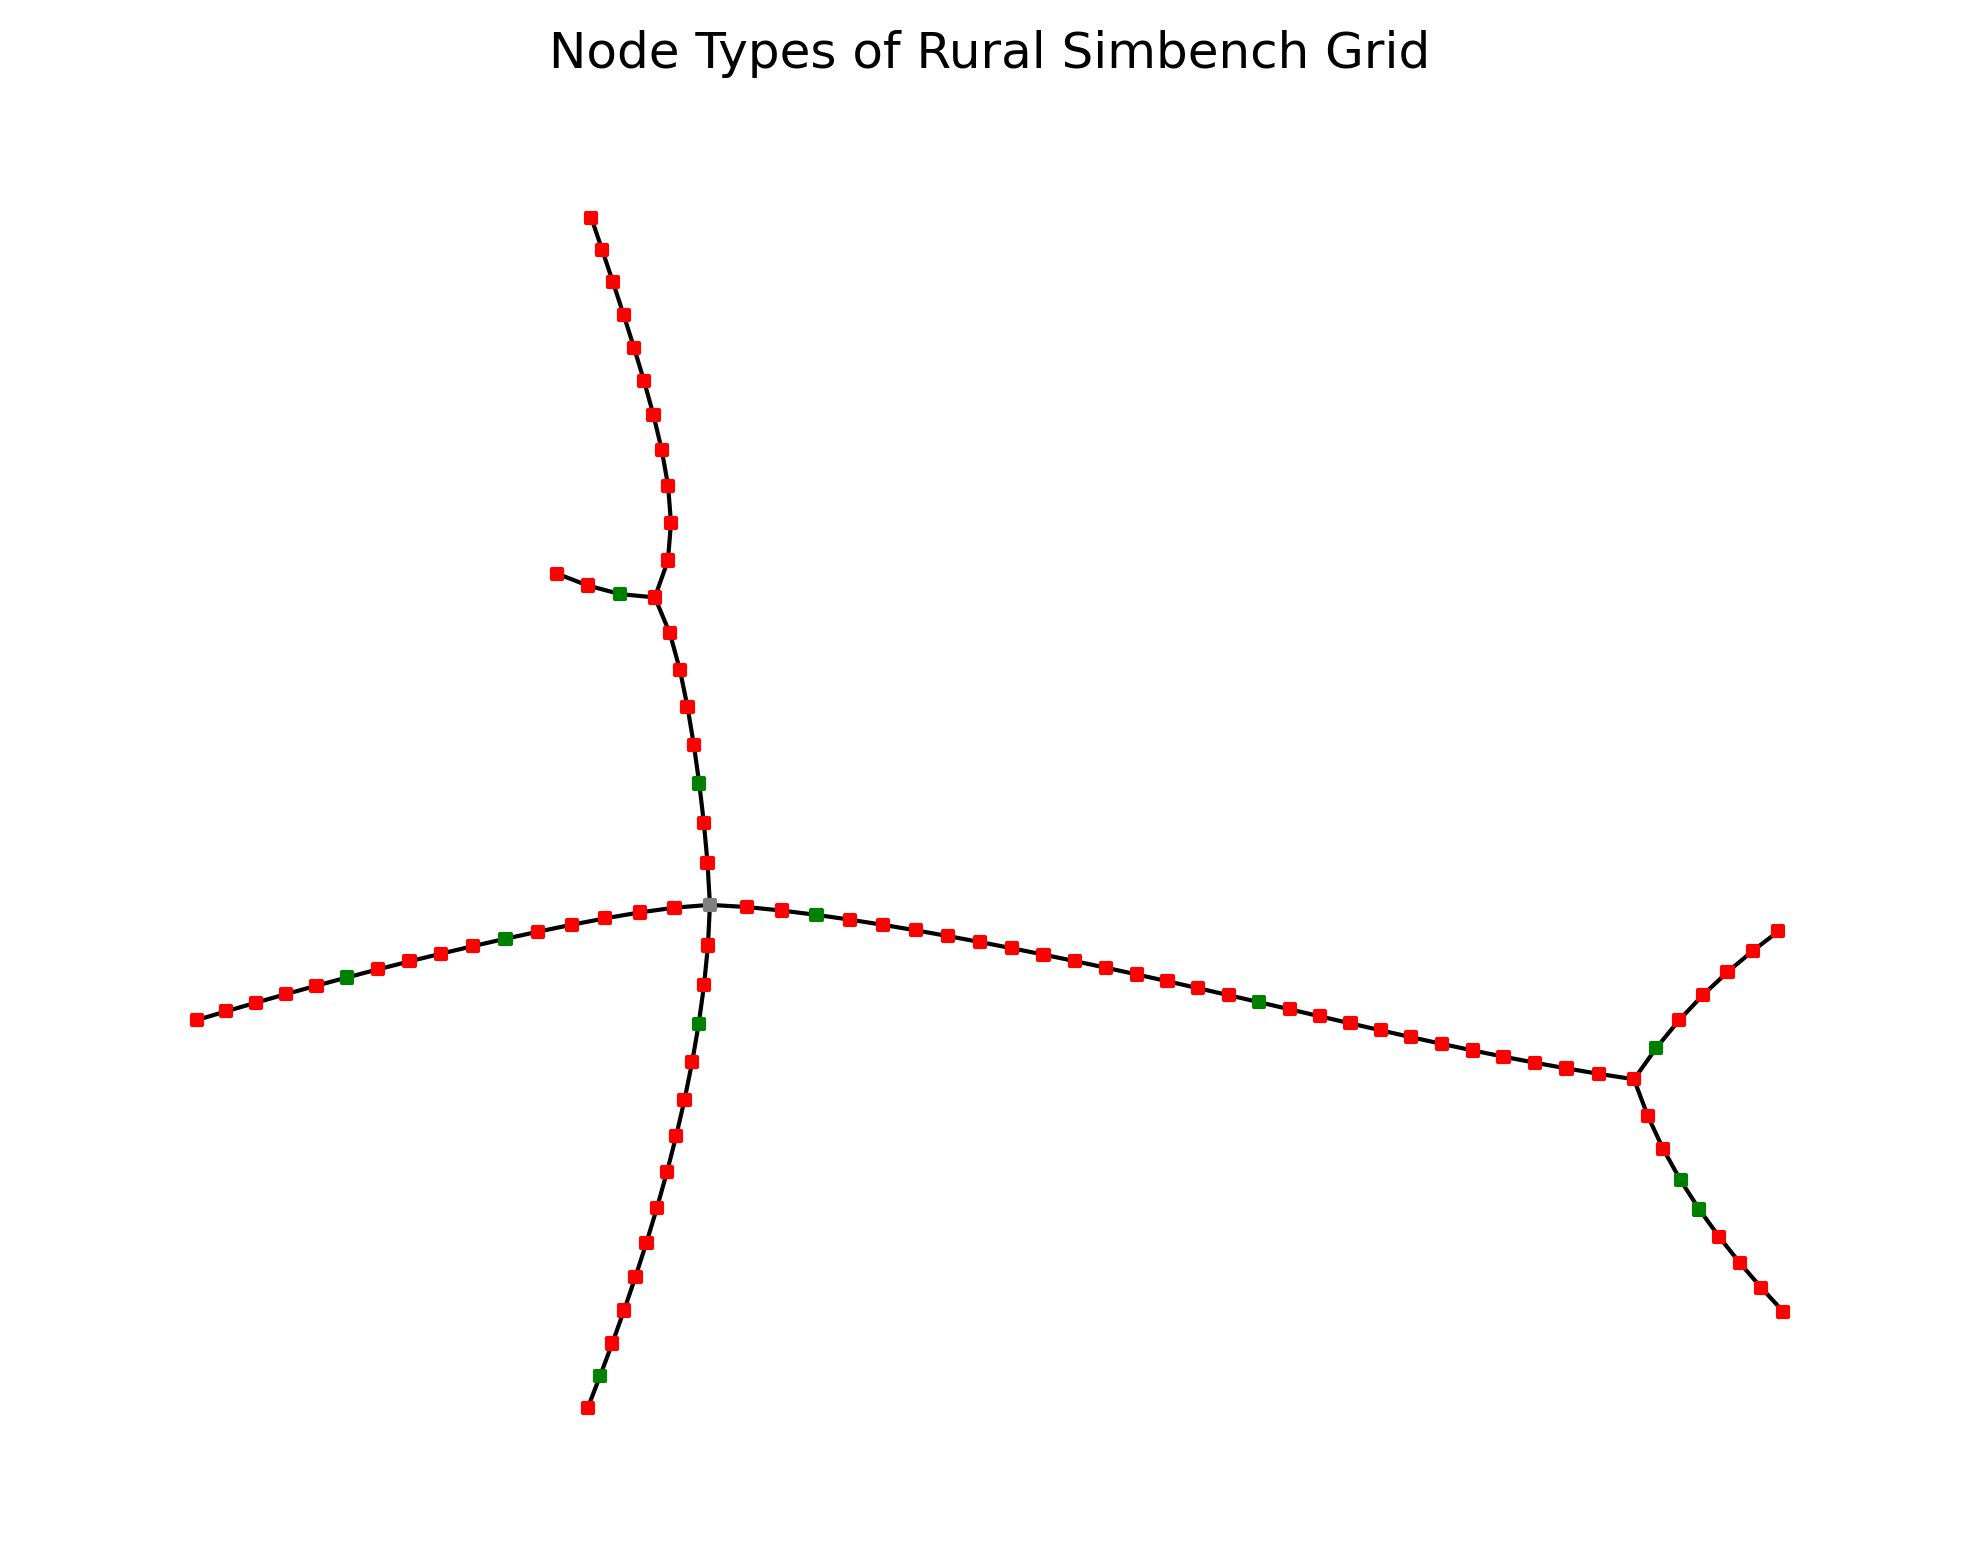
\includegraphics{img/simbench/layout.png}
    \caption{
        Non-geographical representation of the SimBench "1-LV-rural1"
        grid\autocite{simbench}. Nodes with connected transformers are shown
        in \textbf{grey}, households with solar panels in \textbf{green}
        and normal households in \textbf{red}. Only cables with non-zero impedance shown, any nodes
        connected by zero impedance cables have been merged.
    }
    \label{fig:vep:simbench_node_types}
\end{figure}


% The grouping into grids
% Outer world (for geographical locations)
%   Nodes
%   Edges
% Inner world (conducting)
%   Nodes (simple, prosumer, slack)
%   Edges (switches, simple, with impedance, transformers)
% Standard switchstate

\subsection{Grid Load}

To simulate the grid adequately, production and consumption values for
each of the prosumers is needed. VEP provides various different models
to do so ranging form standard load profiles (standardized curves which are adjusted
according to the prosumer's parameters), neural network models trained on historic data,
weather forecast based models and actual real time measurement values\autocite{venios}.\\
\\
Within real low voltage girds, the data available will often be spotty. Not all prosumers
have measurement devices and their measurement frequency is often limited. The most accurate
load modelling data is therefore often a mixture of the sources mentioned above.\\
\\ 
For this work all load timelines will be obtained from Venios through its API. Venios works
closely with the grid operators to make sure these timelines most closely resemble the conditions
in the real grid. This important as these values are being used to monitor the grid and in some
cases trigger active control measures\autocite{venios}. Within this work it is assumed that the data
available through the API is the best data available, which most closely resembles the actual grid load.
Any switch states and their effects on grid parameters will be tested against this data. It can
thus be reasonably assumed that any improvements seen based on this data translate reasonably well
into the real world. 

\begin{figure}[H]
    \begin{subfigure}{.5\textwidth}
      \centering
      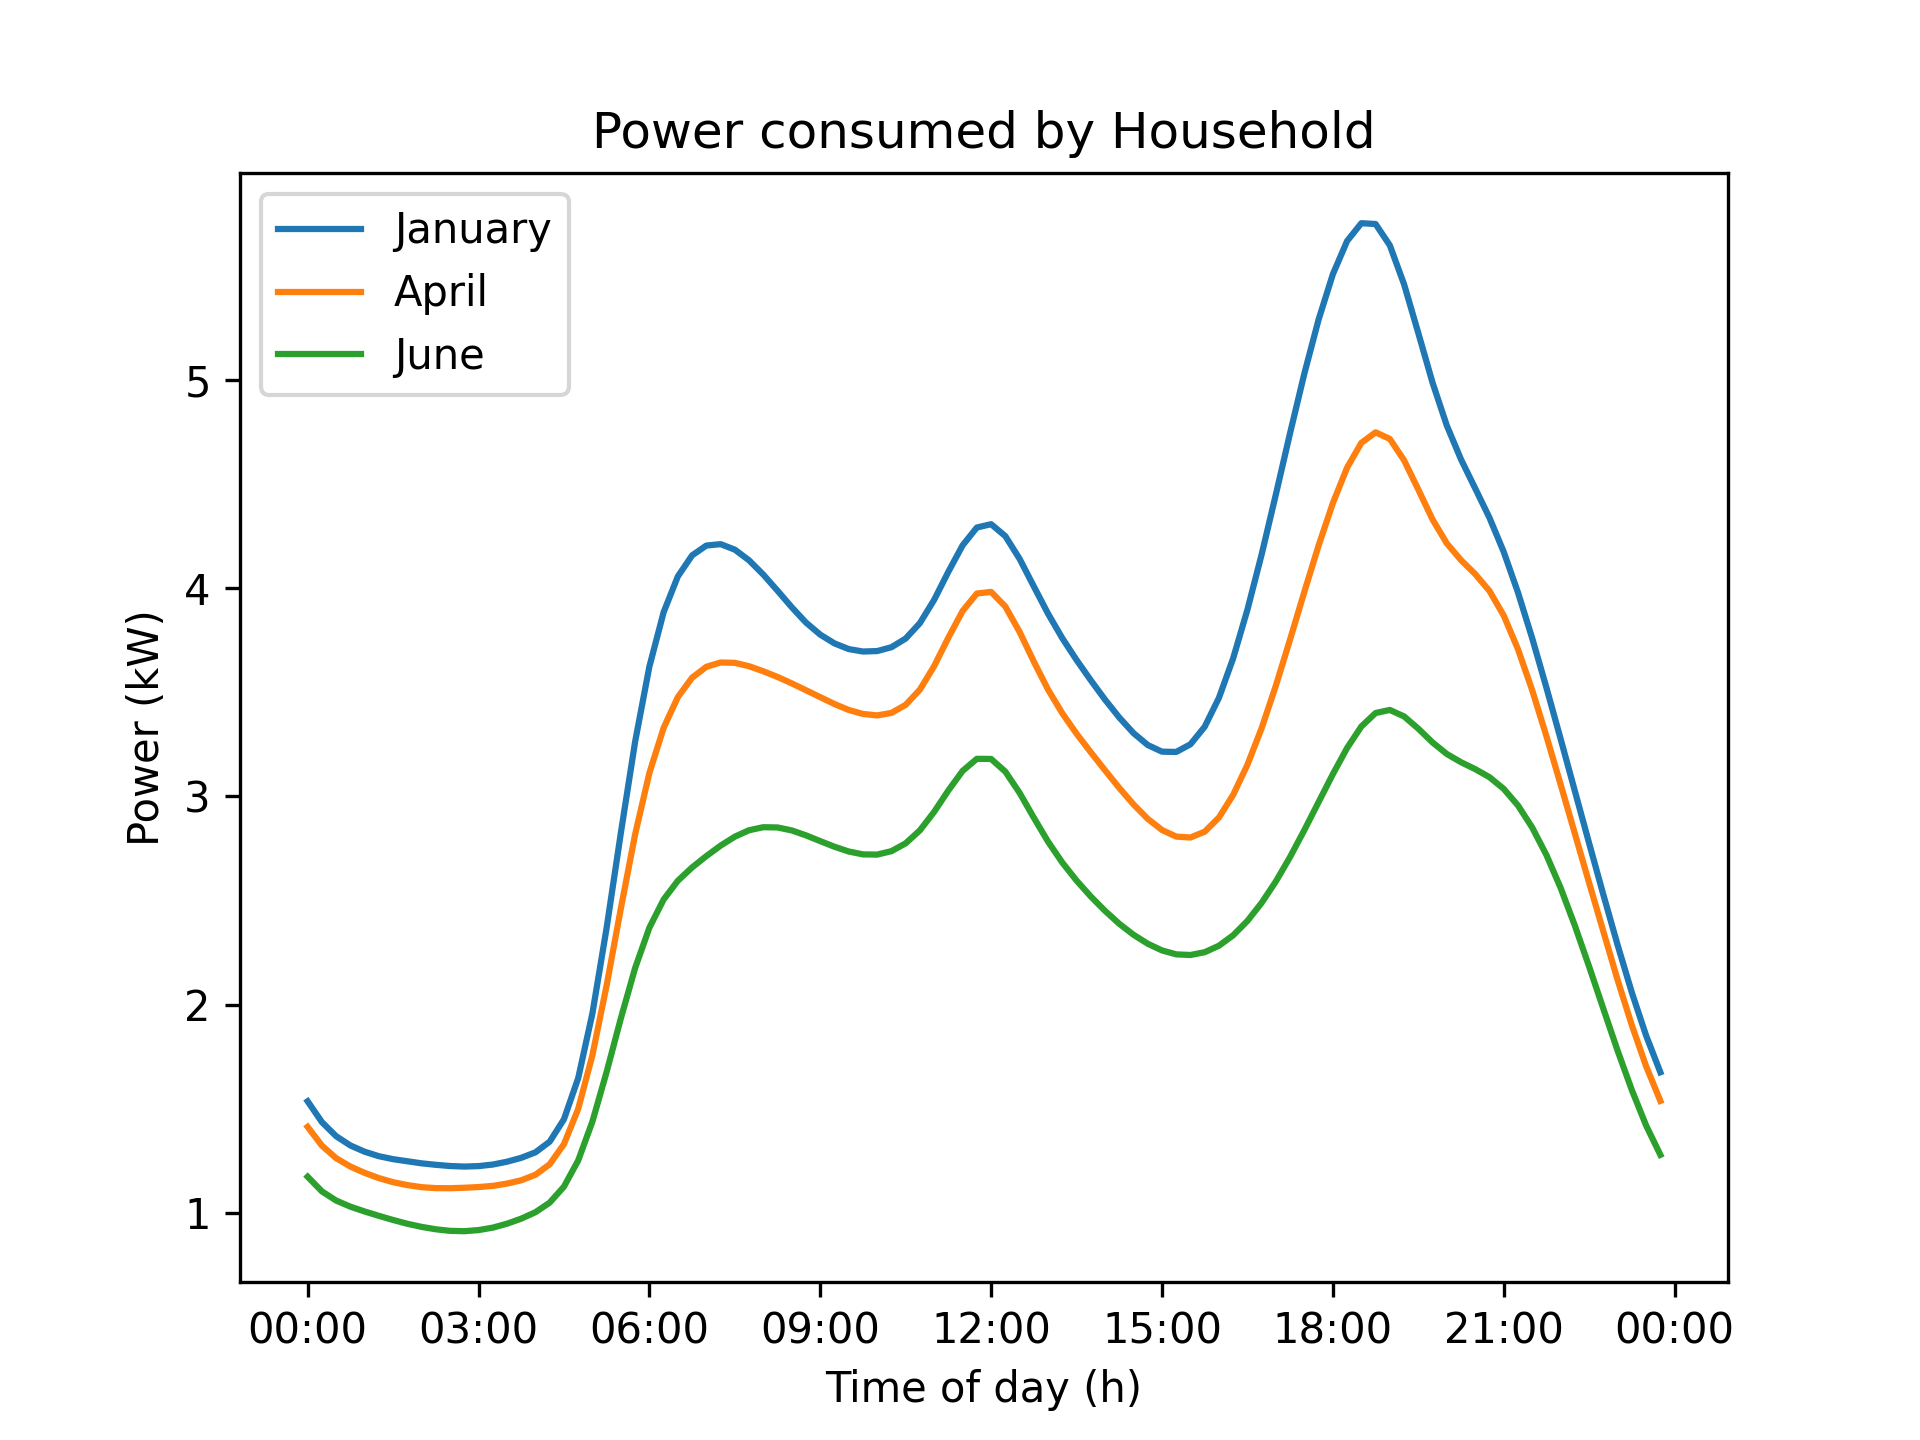
\includegraphics[width=\linewidth]{img/simbench/load_profile_household.png}
      \caption{}
      \label{fig:vep:load_profile_household}
    \end{subfigure}%
    \begin{subfigure}{.5\textwidth}
      \centering
      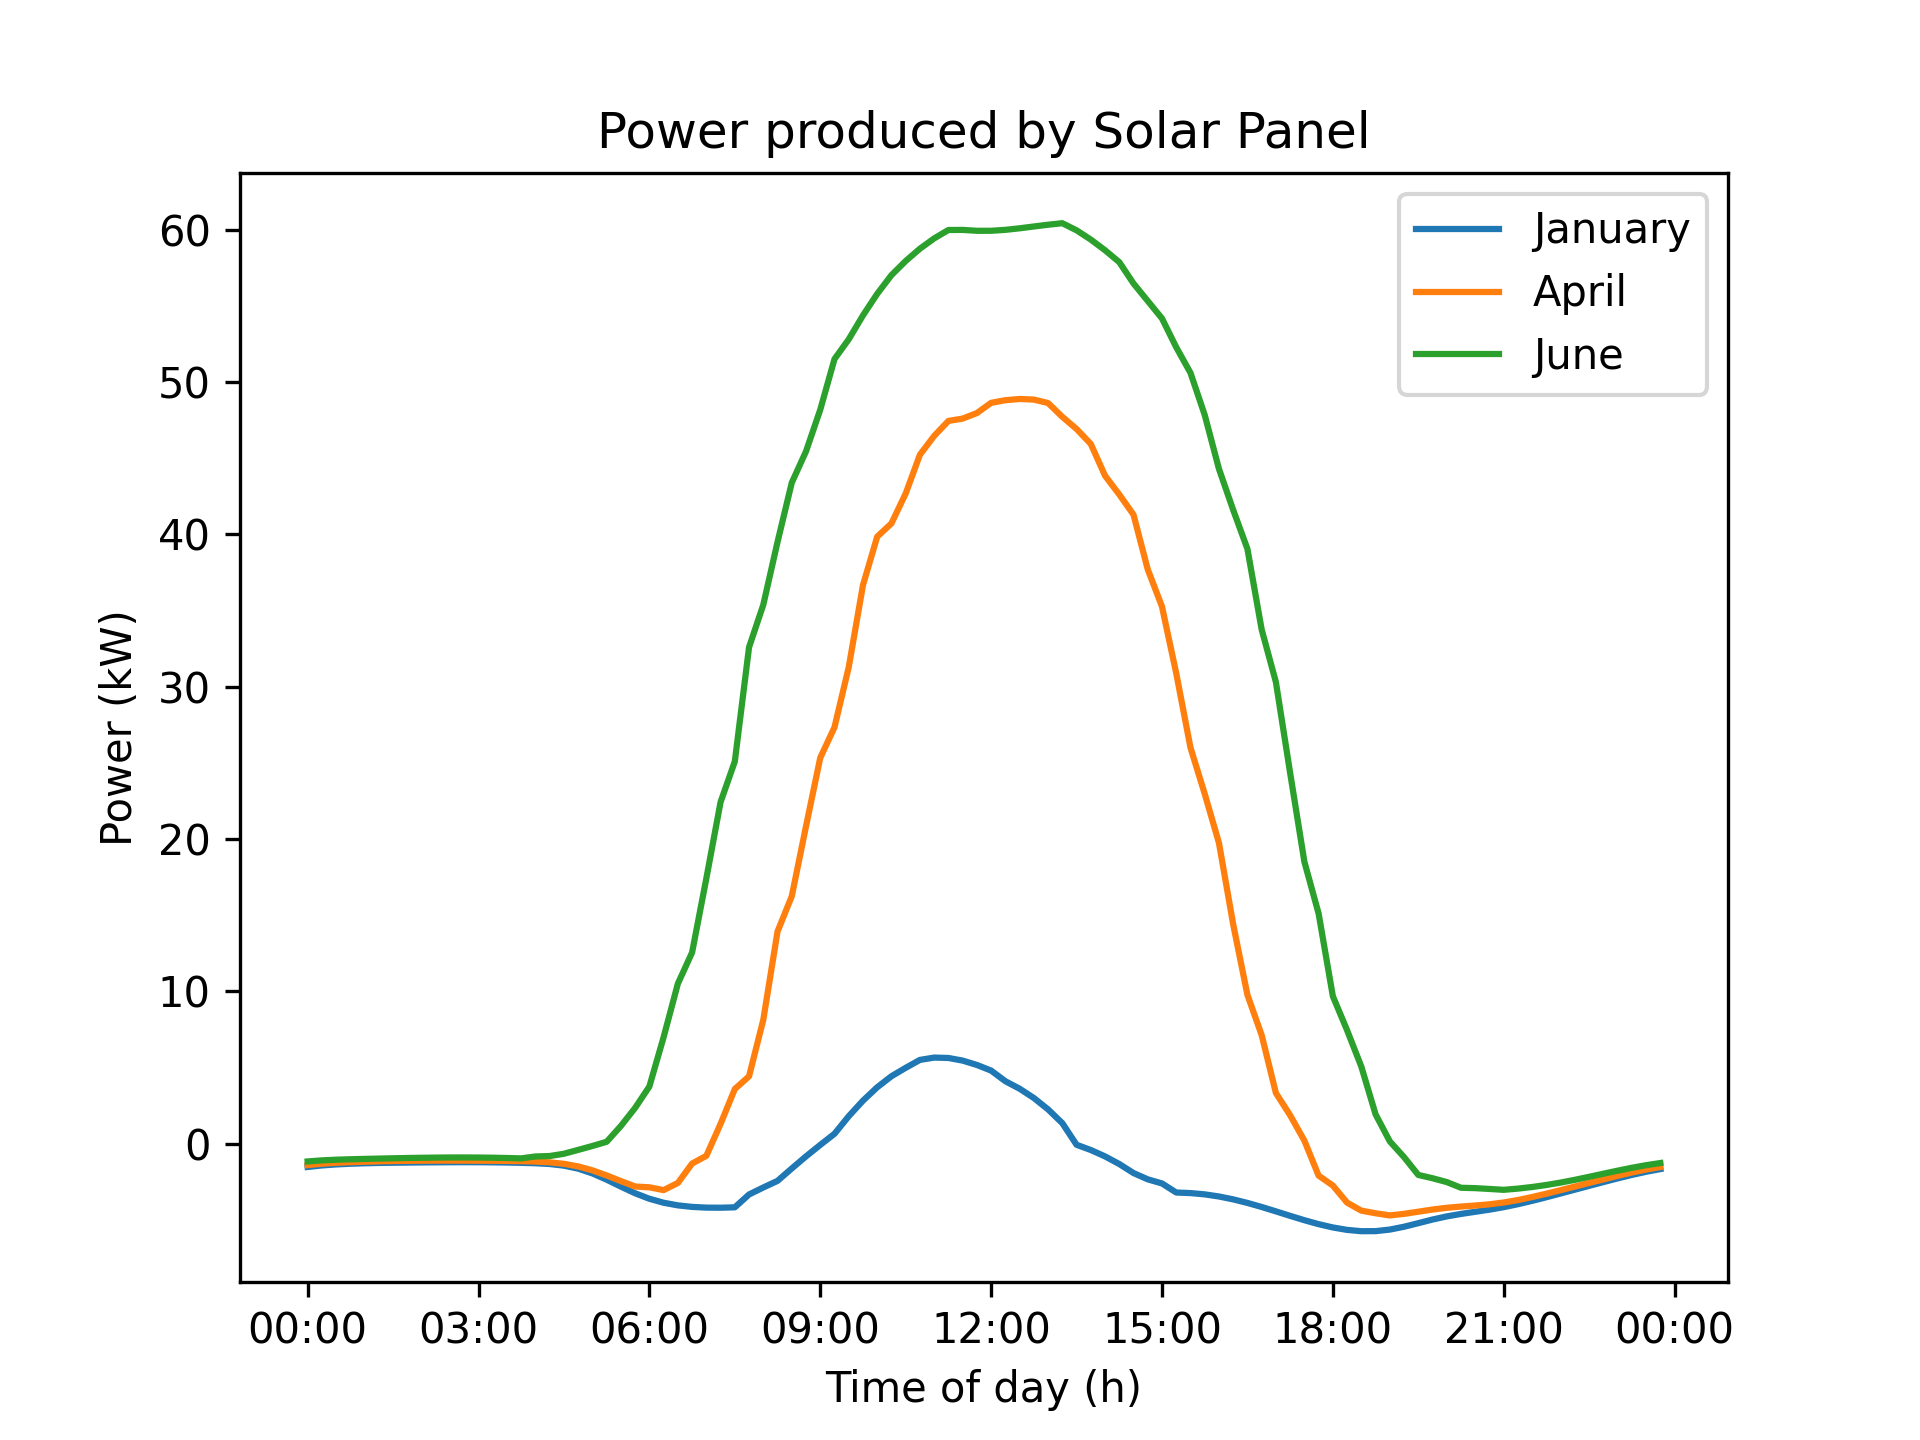
\includegraphics[width=\linewidth]{img/simbench/load_profile_solar.png}
      \caption{}
      \label{fig:vep:load_profile_solar}
    \end{subfigure}
    \caption{Power produced/consumed by a household (a) and a solar panel (b) within a SimBench grid at different times of day and at different times of year. Data is generated by a standard laod profile model within VEP and obtained over API\autocite{venios}}
    \label{fig:vep:load_profiles}
\end{figure}

Figure \ref{fig:vep:load_profiles} shows some example load data obtained from VEP. It can be seen
that power production and consumption varies, widely throughout the day and the year. As a result the grid
might act very differently depending on the season and time. An important question to answer is therefore if
there are swtichstates that are generally better or if the best switch state is highly dependent on
time.\\
\\
Often switches within the grid can only be operated manually\autocite{venios}. Therefore, changing the grid configuration is linked to
some effort and cannot be done very often. If it turns out that there are switch states that are consistently better
a new and improved permanent switch state could be considered. If the best switch state is
however dependent on time, then depending on the scale of improvement, remotely controlled switches might be a worthwhile
investment.